% Chapter Template
%!TEX root=../main.tex
\chapter{1-D Memristor Simulation} % Main chapter title

\label{Chapter6} % Change X to a consecutive number; for referencing this chapter elsewhere, use \ref{ChapterX}

\lhead{Chapter 6. \emph{Memristor Simulation}} % Change X to a consecutive number; this is for the header on each page - perhaps a shortened title

\begin{doublespace}

A numerical method for a coupled ionic-electronic device simulation \tjsr{is}{was} developed and tested in previous chapters based on drift-diffusion equations and finite difference. This chapter introduces a 1-D approximation for \tjs{a} 2-D cross section of the memristor. Then 1-D simulations of a memristor are shown under various conditions.
\section{1-D Memristor Approximation}

For \tjs{the} 1-D simulation it is assumed that there are always more than enough ions to saturate the PEDOT:PSS so the electrolyte is modeled as an infinite source/sink of ions. The top boundary of the electrolyte is assumed to be charge neutral at all times which provides a mechanism for moving ions in and out of the system. This way the movement of ions near the surface of the PEDOT can still be captured without having to simulate the ion movement for the entire electrolyte solution which is variable in size. This assumption is not used for 2-D simulations since the electrolyte is fully simulated.
 
The horizontal cross section from figure \ref{MemStc} has the most crucial elements of the memristor but its simulation in 1-D is not straightforward. This cross section through the PEDOT does not include the vertical movement of the lithium ions. Without this effect, PEDOT:PSS is just a regular conductor with a uniform current density. In order to overcome this problem a generation/recombination term for lithium ions (calculated at every time step) is added to capture the vertical movement in addition to the regular drift diffusion equations which represents the horizontal movement. This generation/recombination term can be symbolized as a current source connected to all the nodes (figure \ref{MemStc15}). Perchlorate ions are not included in the simulation since they do not move into the PEDOT.

 
\begin{figure}[!htp]
\centering
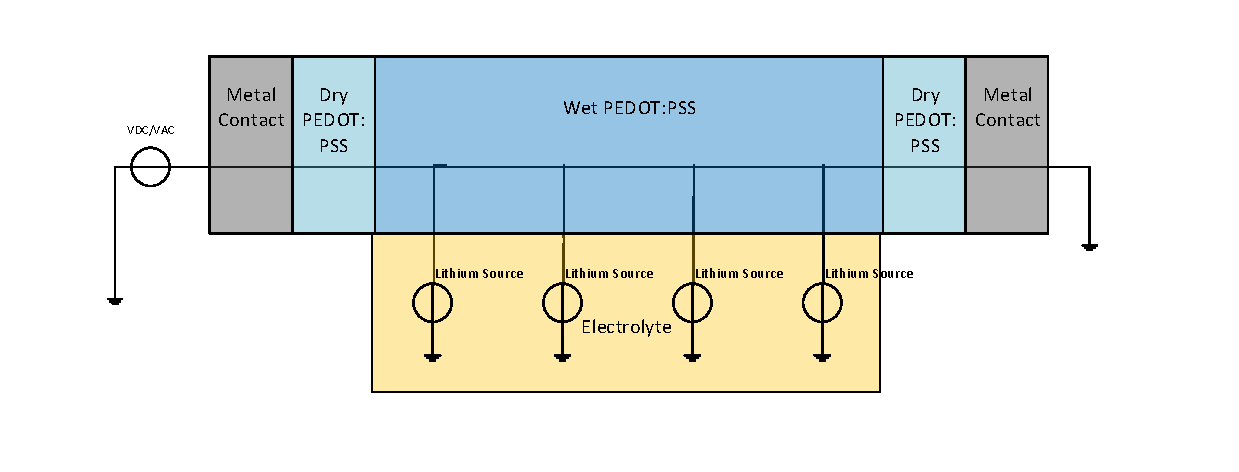
\includegraphics[scale=0.74]{1DMem}
\caption{1-D Memristor Model} 
\label{MemStc15}
\end{figure}


The lithium source has two different terms, one for drift and another one for diffusion. It was assumed that the concentration of lithium is always constant in the electrolyte. This way the vertical diffusion current density can be calculated using the difference between the lithium density in PEDOT:PSS and electrolyte,
\begin{equation}
J_{diff} = K_1 q D  \frac{n - n_c}{\Delta x}
\end{equation}
\textit{n} and \textit{$n_c$} are lithium densities in the PEDOT:PSS and electrolyte respectively. \textit{$K_1$} is a fitting parameter that can be adjusted based on experimental results. For the drift term an electric field is estimated between the PEDOT:PSS and the electrolyte. First the potential of the electrolyte is assumed to be the average potential of both metal contacts, 
\begin{equation}
V_{el} =  \frac{V_L+V_R}{2}
\end{equation}
Where $V_L $ and $V_R$ are the electric potentials of the left and right metal contacts. Then a vertical electric field is calculated using the electrolyte and the instantaneous potential of the PEDOT:PSS at different positions, 
\begin{equation}
E_{y} =  \frac{V_{el}-V }{\Delta x}
\end{equation}
Finally a drift current for lithium ions is calculated using the estimated electric field, 
\begin{equation}
J_{drift} = \begin{cases}
        K_2 q \mu n_c E_y  & \text{for} \;  E_y>0  \\
        K_2 q \mu n E_y   &  \text{for} \;  E_y<0  \\
     \end{cases}
\end{equation}
\textit{$K_2$} is a fitting parameter for drift that can be adjusted based on experimental results. When the electric field is positive, lithium ions are being pulled into the PEDOT:PSS and when it is negative they are being absorbed by the electrolyte. Finally the drift and diffusion current densities can be added to calculate the net lithium current density for the lithium sources,
\begin{equation}
J_{s} =  J_{drift}+J_{diff}
\end{equation}
For both drift and diffusion the horizontal movement of lithium ions inside the electrolyte is not modeled. The 1D model therefore models the flow of Lithium in and out of the PEDOT as a strictly vertical 1D flow.


\clearpage
\section{1-D Memristor Simulations}

The following simulations are made based on the memristor approximations discussed above. The first two simulations are repeated in the next chapter using a 2-D drift diffusion and Poisson solver which captures a broader range of physical effects. Both approaches are compared in order to understand their advantages and disadvantages under different circumstances.

\subsection{1-D Memristor Simulation Using a Potential Pulse Train}
  
For the following simulation a potential pulse train, slow enough to let the memristor reach steady state \tjs{between transitions}, is applied at the left contact.
\begin{figure}[!htp]
\centering
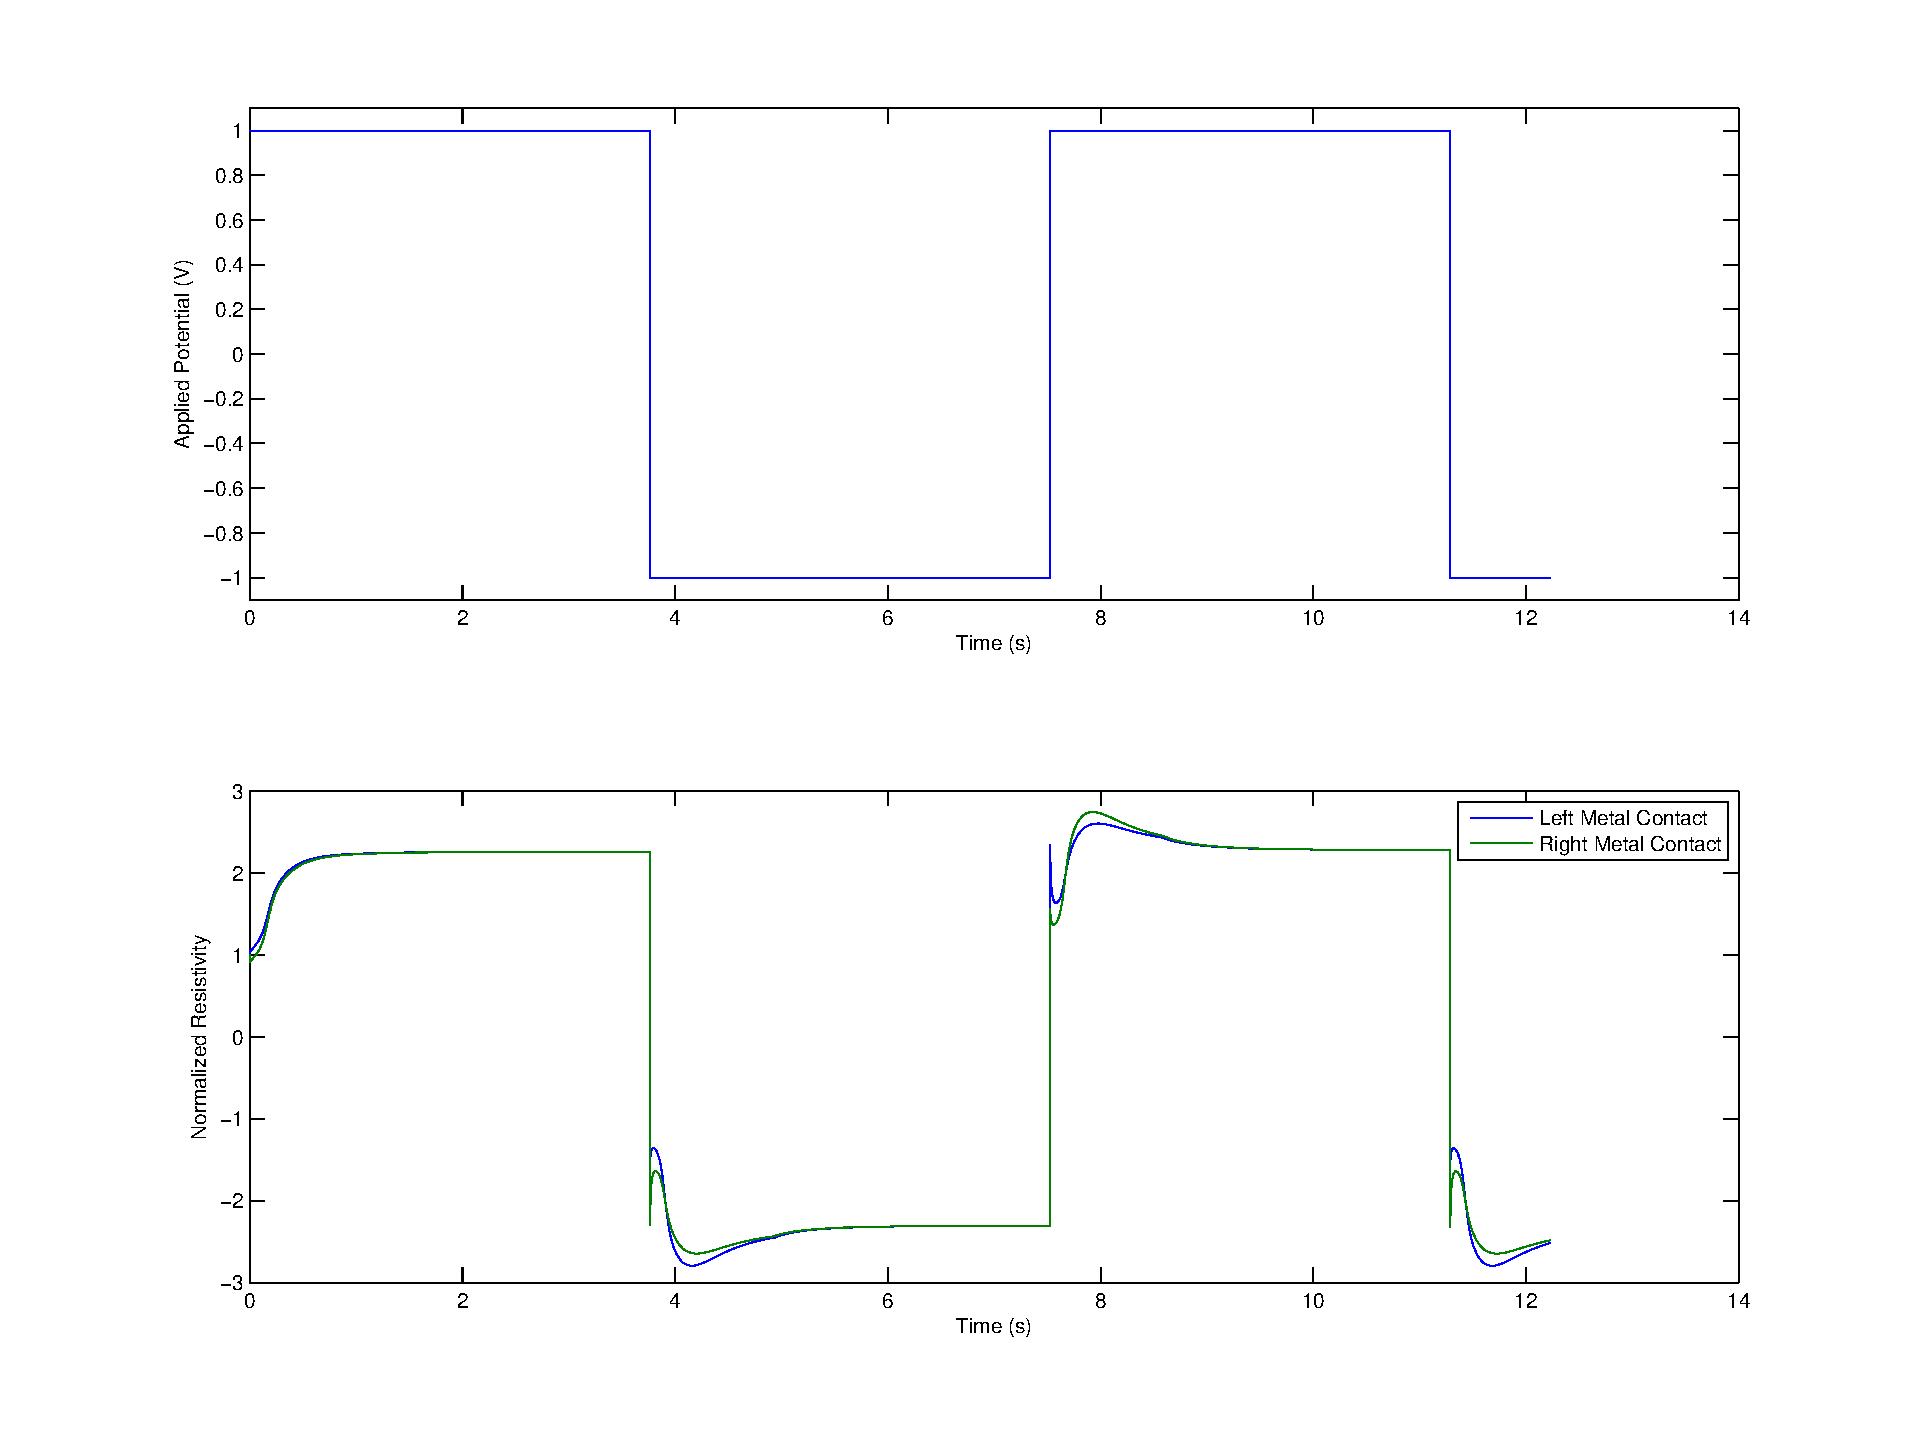
\includegraphics[scale=0.55]{1DMemPulseTrain}
%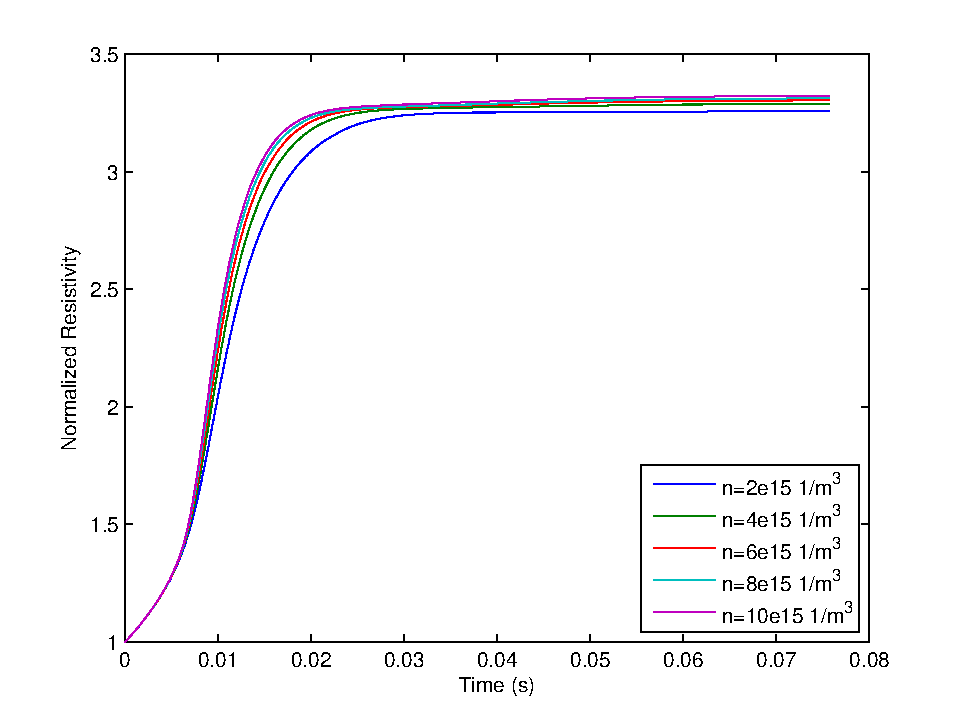
\includegraphics[scale=0.60]{Ex5DCResistivity}
\caption{Change in current density over time due to applied potential} 
\label{MemResTrain}
\end{figure}
\tjsr{Following plot}{Plot} \ref{MemResTrain} shows the current density output for both contacts separately. As expected the current density of the device decreased as the lithium ions move in. Additionally, it can be seen from the graph \ref{MemResTrain} that the current density output from left and right contacts are not always the same over the duration of the simulation. This is due to the PEDOT:PSS layer losing holes on one side and gaining holes on the other side which produces a difference in the measured current density between contacts. The scale of the difference depends on the rate of change in lithium movement on either side.

The current density in figure \ref{MemResTrain} shows a sudden increase when the potential is switched from 1 to 0 and vice versa. This sudden increase occurs because of the accumulation of lithium ions at the wet/dry interface which creates an opposing potential to the applied potential (see figure \ref{MemEss}). When the electric potential changes suddenly, \tjs{the} previously opposing electric field now helps the movement of holes and lithium towards the other end of the device. This additional electric field momentarily increases the current density output of the device.

\begin{figure}[!htp]
\centering
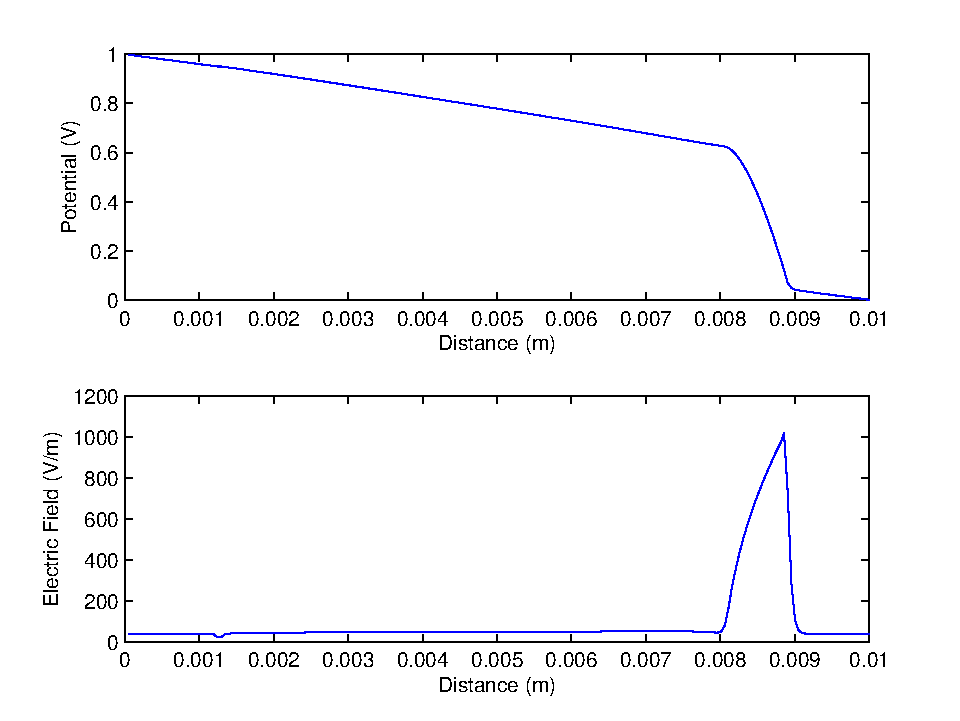
\includegraphics[scale=0.70]{1DMemPot_Efield_SS}
\caption{Potential and electric field at steady state} 
\label{MemEss}
\end{figure}

Figure \ref{MempLi} demonstrates the replacement of holes by lithium ions over time which directly effects current density.  As lithium ions get pulled in from the electrolyte toward the contact they accumulate inside the PEDOT:PSS. Concurrently hole density decreases in areas where lithium accumulates. The decrease in the hole density in the PEDOT:PSS decreases the current density output of the memristor. This change in current density over time is illustrated in figure \ref{MemResTrain}.

\begin{figure}[!htp]
\centering
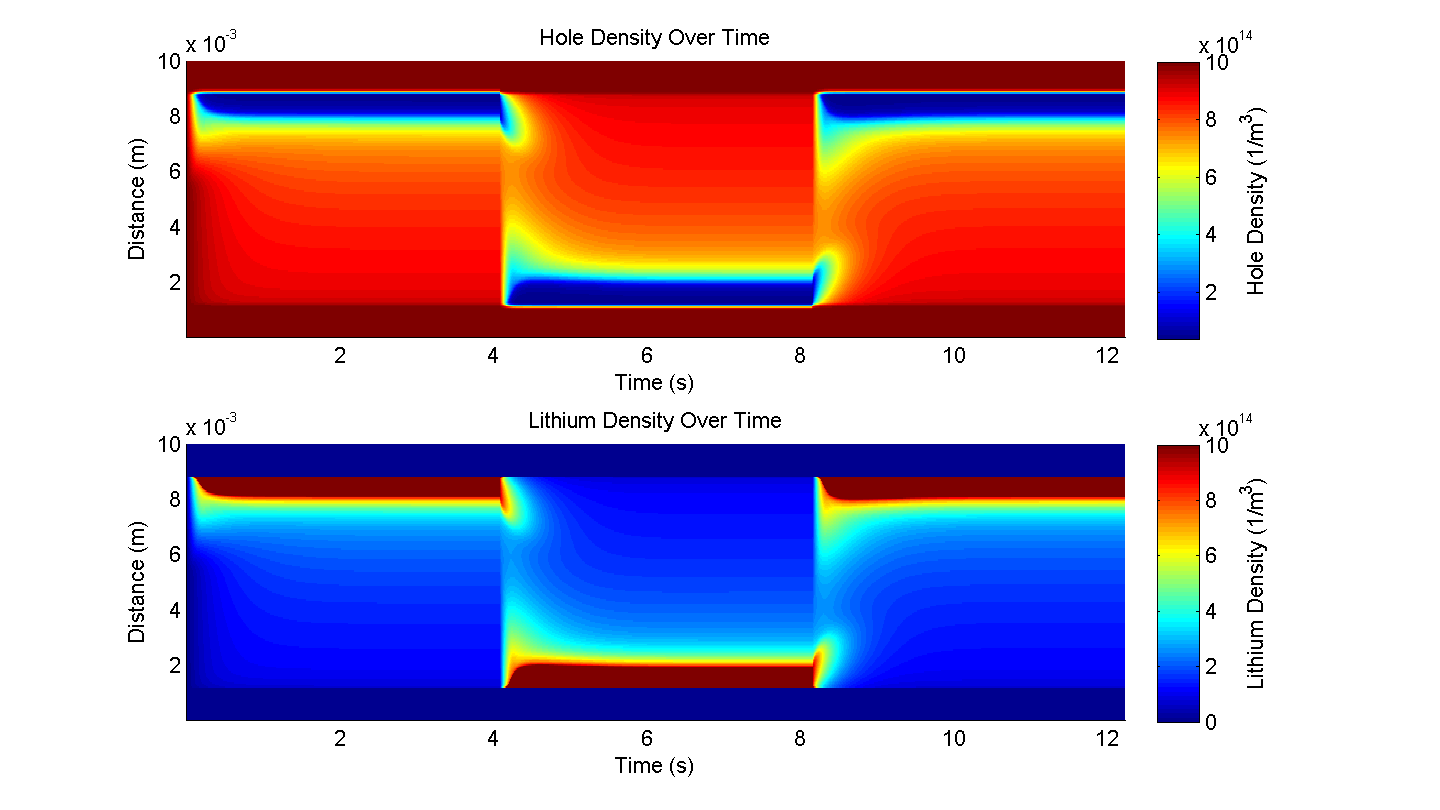
\includegraphics[scale=0.65]{1DMemDensityOverTime}
%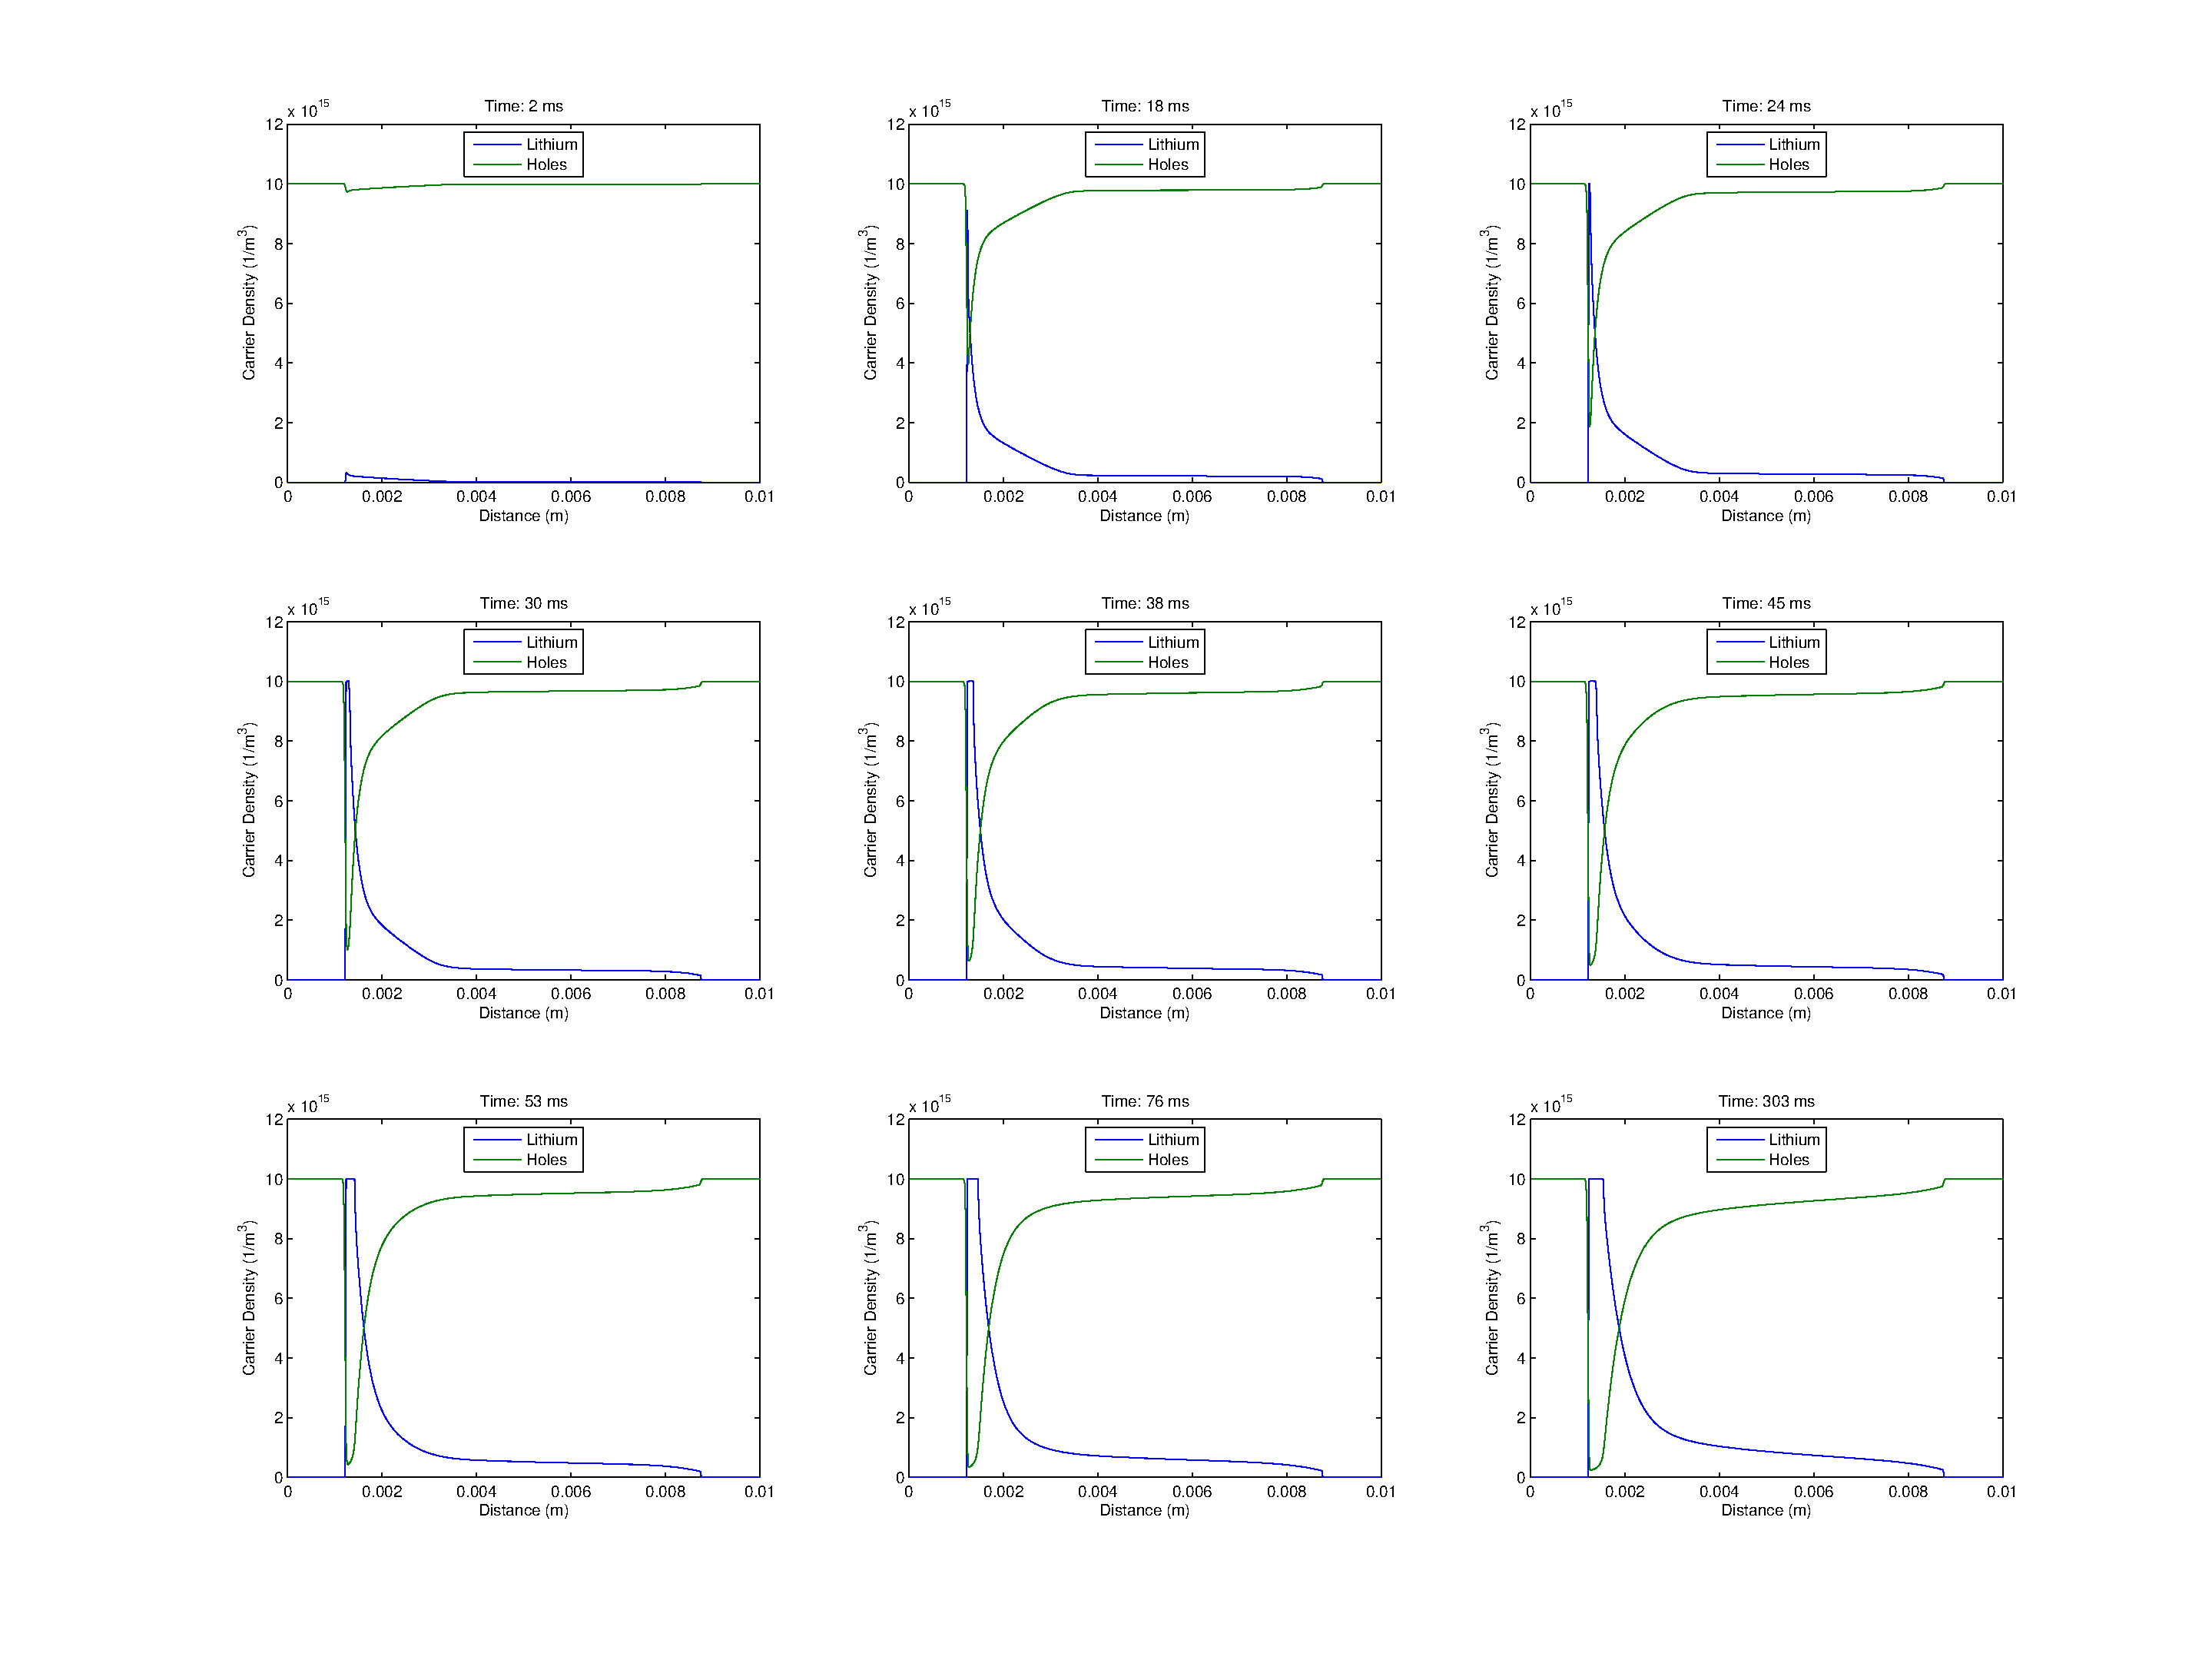
\includegraphics[scale=0.40]{Ex5pNp_Time1}
\caption{Lithium and hole density distribution over time} 
\label{MempLi}
\end{figure}

It is important to note that lithium ions are free to move in \textit{x} and \textit{y} directions. In figure \ref{MempLi} it can be seen that after the potential is switched as the lithium density moves from  side to the other. Most of the lithium movement happens through the exchange of ions between PEDOT:PSS and the electrolyte since the distance between them is far less than the length of the PEDOT. So most of the lithium ions, traveling from the positive to the negative contact, are pulled into the electrolyte before they reach the other side. Near the negative contact lithium ions are quickly pulled into the PEDOT:PSS and accumulate at the wet/dry interface. 

By examining the hole/lithium density plots of the PEDOT:PSS it is possible to conclude that it is composed of 3 distinct regions. 2 dry regions, where there is no contact with the electrolyte, have constant uniform resistance. Between these two resistances there is a variable non uniformly distributed resistance controlled by hole/lithium density and hole mobility. So this model captures the main characteristic of the memristor which is a variable charge dependent resistance where the resistance at any time depends on the past of the device. Following equation gives the total resistance/memristance for the memristor model developed for this thesis:

\begin{equation}
\centering
M(q(t))_{tot}=2R_{dry}+R(Li,p,\mu_{hole})
\end{equation}

The minimum resistance of this device is just the total resistance of the PEDOT:PSS without the lithium ions. The maximum resistance depends on different factors such as applied potential and the distribution and density of lithium ions inside \tjs{the} PEDOT:PSS.

\clearpage
\subsection{1-D Memristor Simulation Using a Sinusoid}

The memristor with a pulse train simulation shows the change in the current density over time due to an applied potential but it does not clearly demonstrate the memory effects. The memory effect of the memristor can be clearly demonstrated in an I-V curve using a sinusoidal potential. Following four graphs (figure \ref{Bowtie}) are created using an AC potential with different frequencies at the contacts. All the plots show that current density can have more than one value for the same potential at different times. This means that simulated memristor's past state\tjsr{s}{} affects its present output, therefore the device has \tjsr{a}{} memory. There is \tjsr{a pinch in the current for negative applied potential}{an asymmetry in the current curve} because it is measured from one contact which has relatively low change in resistance for a period of time during transient simulation. 

\begin{figure}[!htp]
\centering
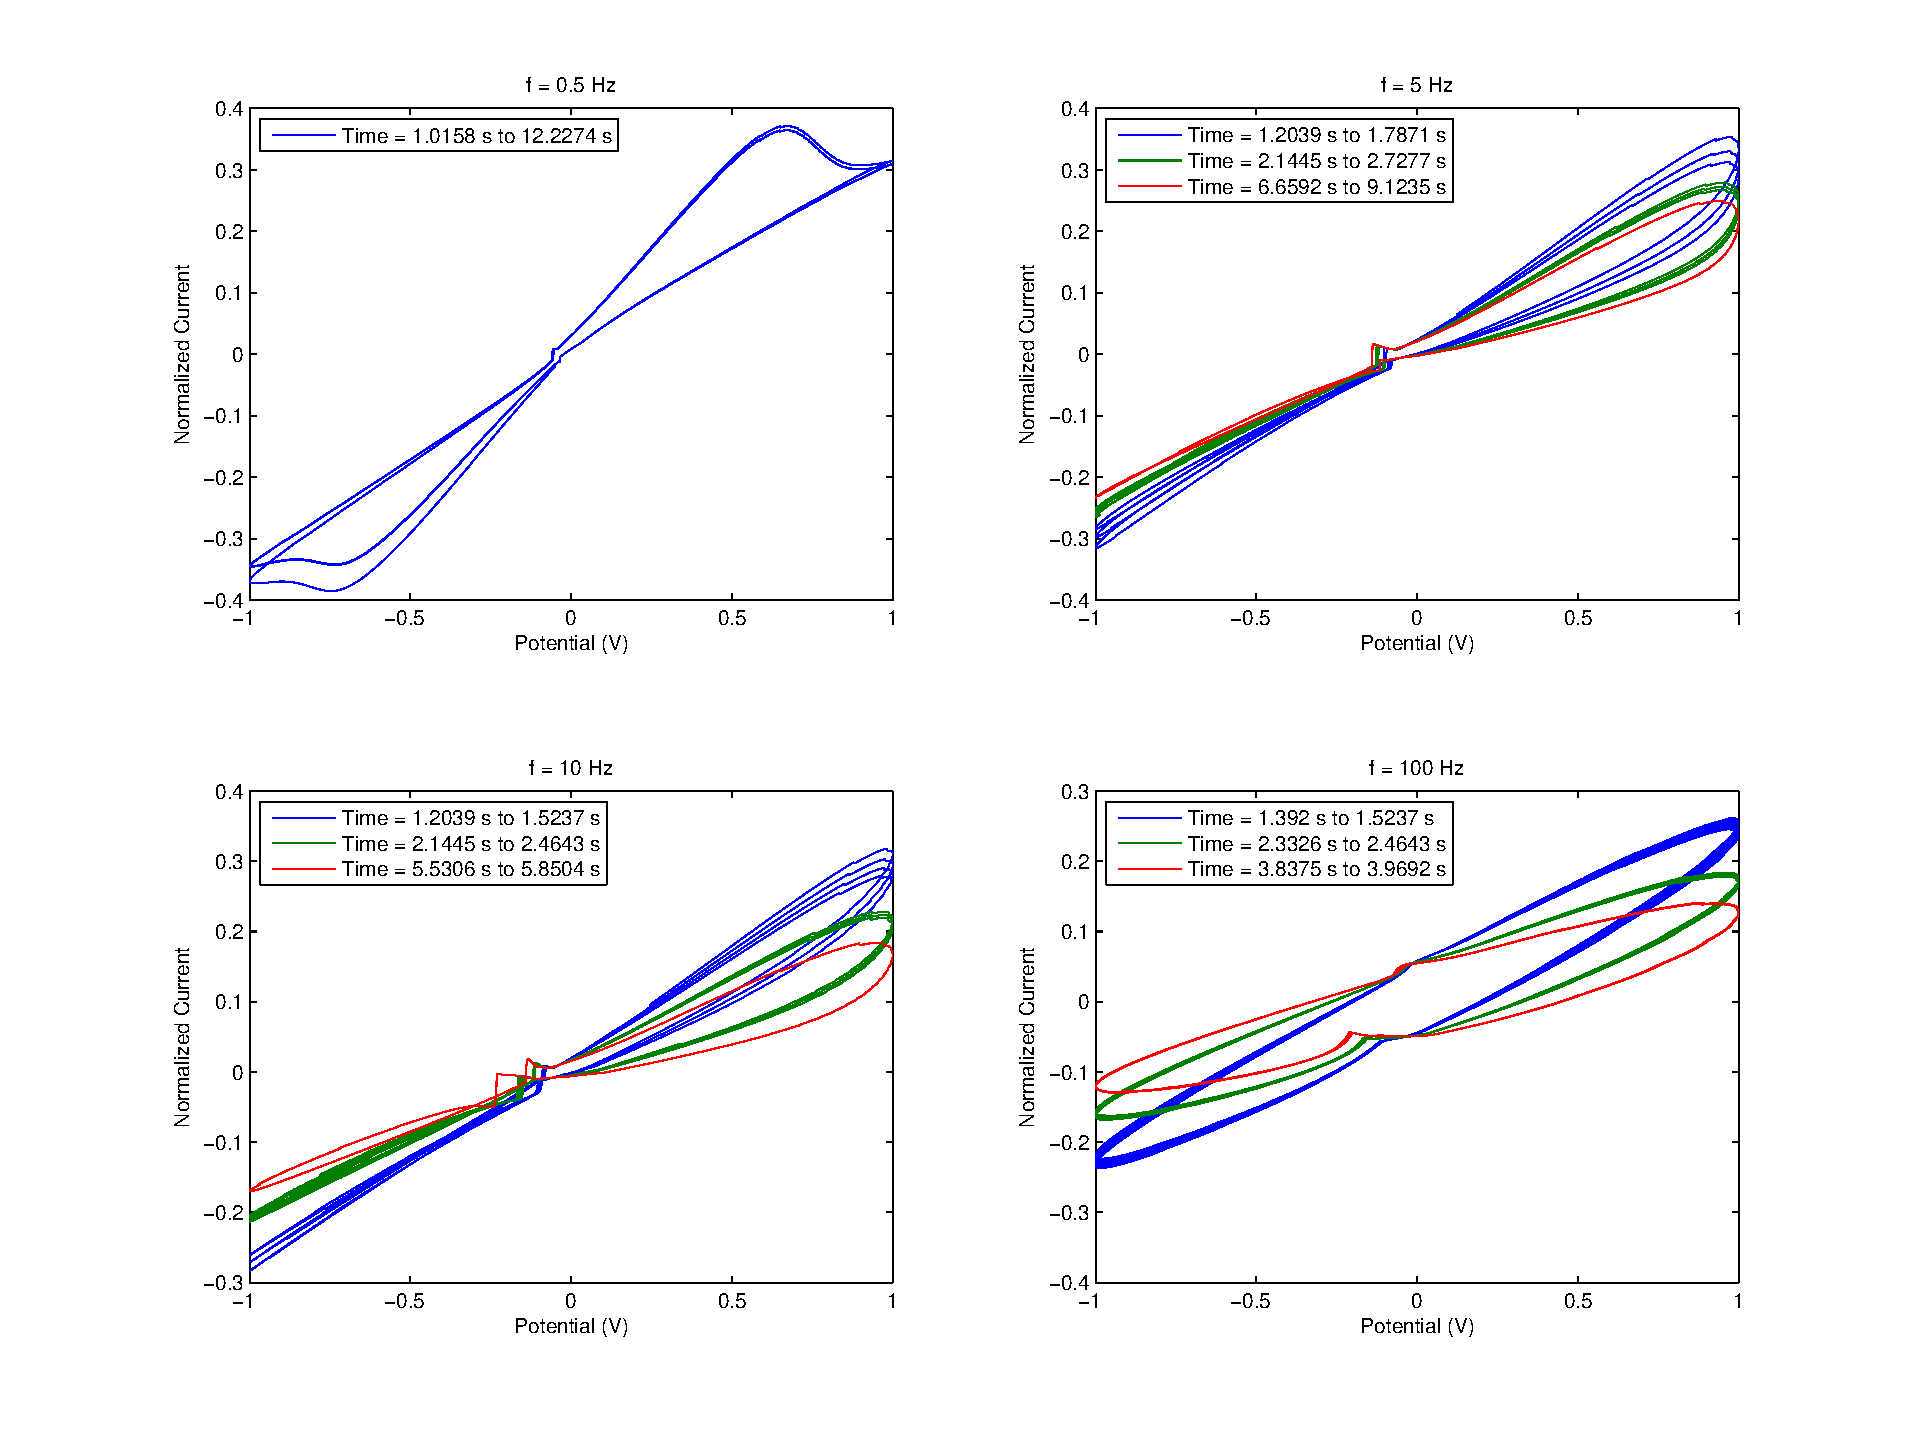
\includegraphics[scale=0.43]{BowtiefAll}
\caption{Normalized Current vs. applied potential at different frequencies} 
\label{Bowtie}
\end{figure}

The sudden changes in current around 0 V can be attributed to the density limiting mechanism for lithium. Instead of a slowdown in the movement of lithium ions near maximum density, the current flow into that region is completely blocked. Even though this makes the lithium density more responsive to changes, \tjsr{sudden movement block}{a sharp block in the flow} combined with large time steps can result in fast changes which can be directly seen as abrupt changes in the hole/lithium current density during transient simulations.  

The following plots (\ref{BowtieCurr}) show that, at first, there is a drop in the average current for all frequencies \tjsr{since lithium diffusion is greater than lithium drift}{as the lithium initially flows into the PEDOT:PSS}. This transient effect disappears once enough lithium settles into the PEDOT:PSS \tjs{to establish a stable distribution of lithium}. 

\begin{figure}[!htp]
\centering
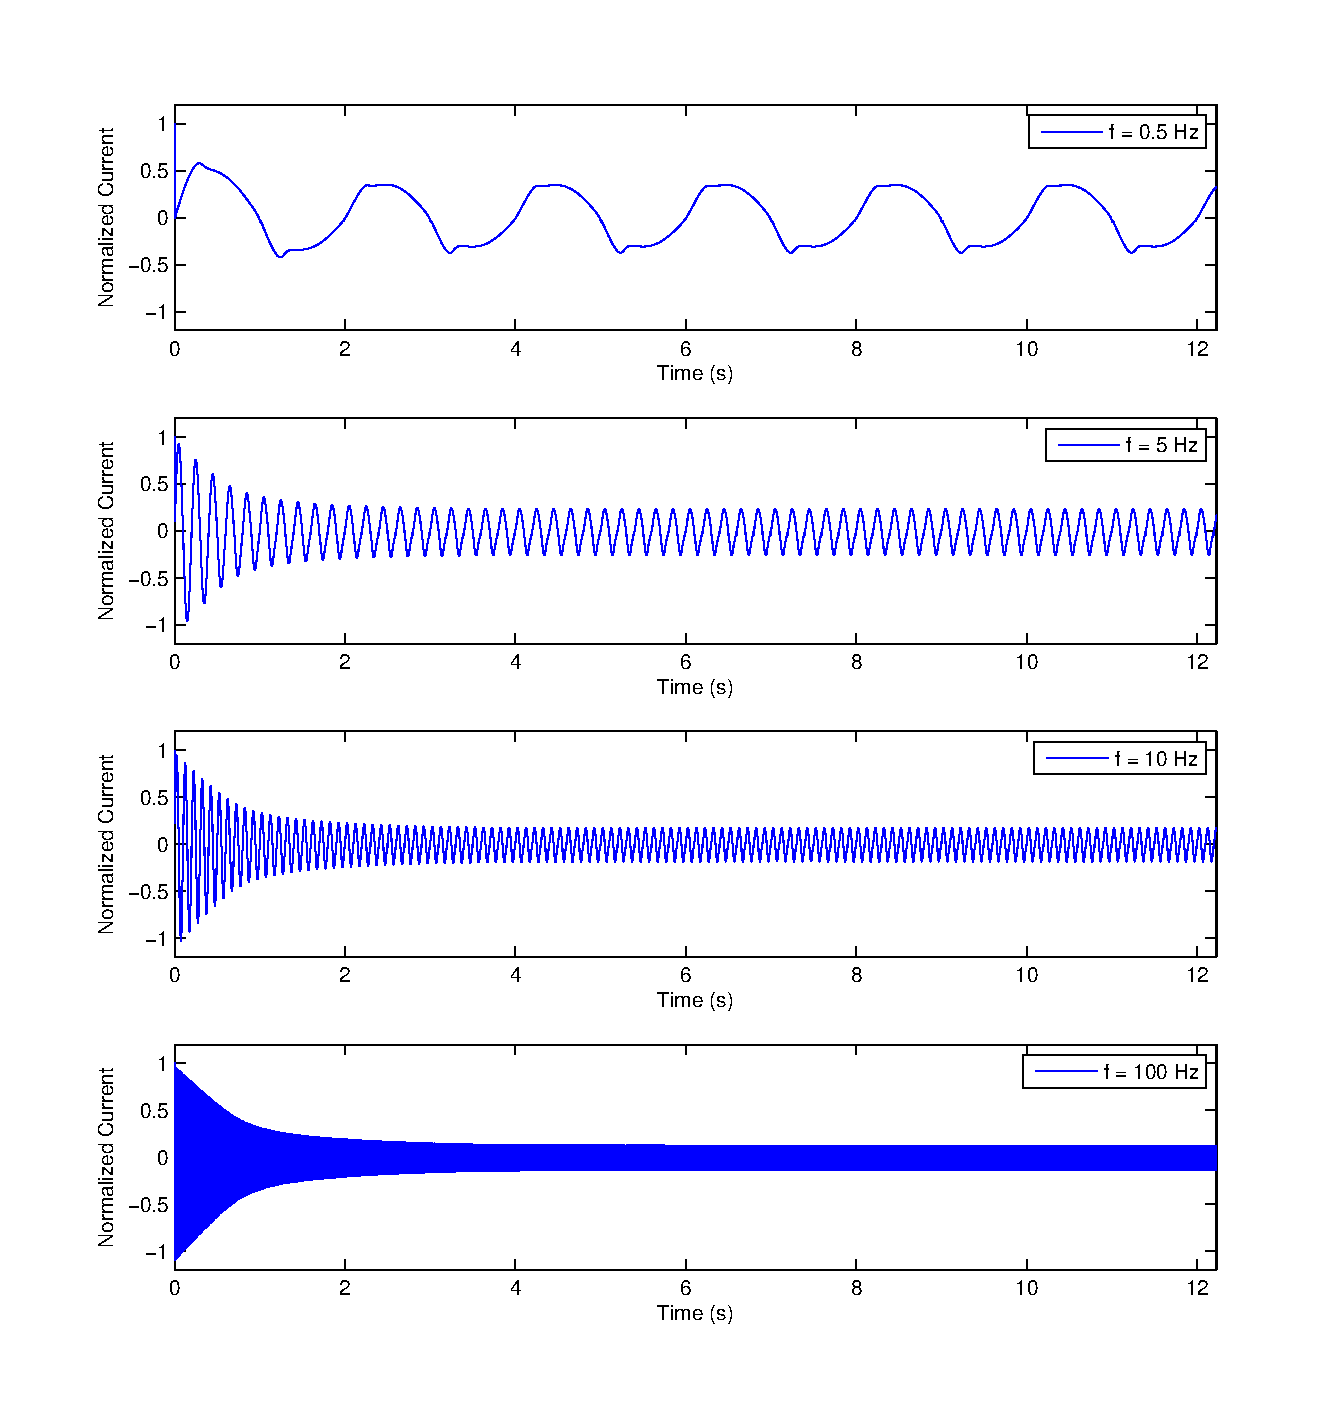
\includegraphics[scale=0.51]{BowtieCurr4f}
\caption{Normalized current over time} 
\label{BowtieCurr}
\end{figure}

Figures \ref{Bowhole} and \ref{Bowli} show the changes in the hole and lithium density in PEDOT:PSS over time. A visual comparison of the plots show that changes in the lithium density are tied to the changes in the hole density. As the frequency increases lithium diffusion becomes more dominant than lithium drift. At 100 Hz lithium drift due to the applied potential is barely present. Since the ions do not create a visible impact on the hole density, the resistivity of the device remains constant over time. This means that the memristor model behaves like a regular resistor at high frequencies.


\begin{figure}[!htp]
\centering
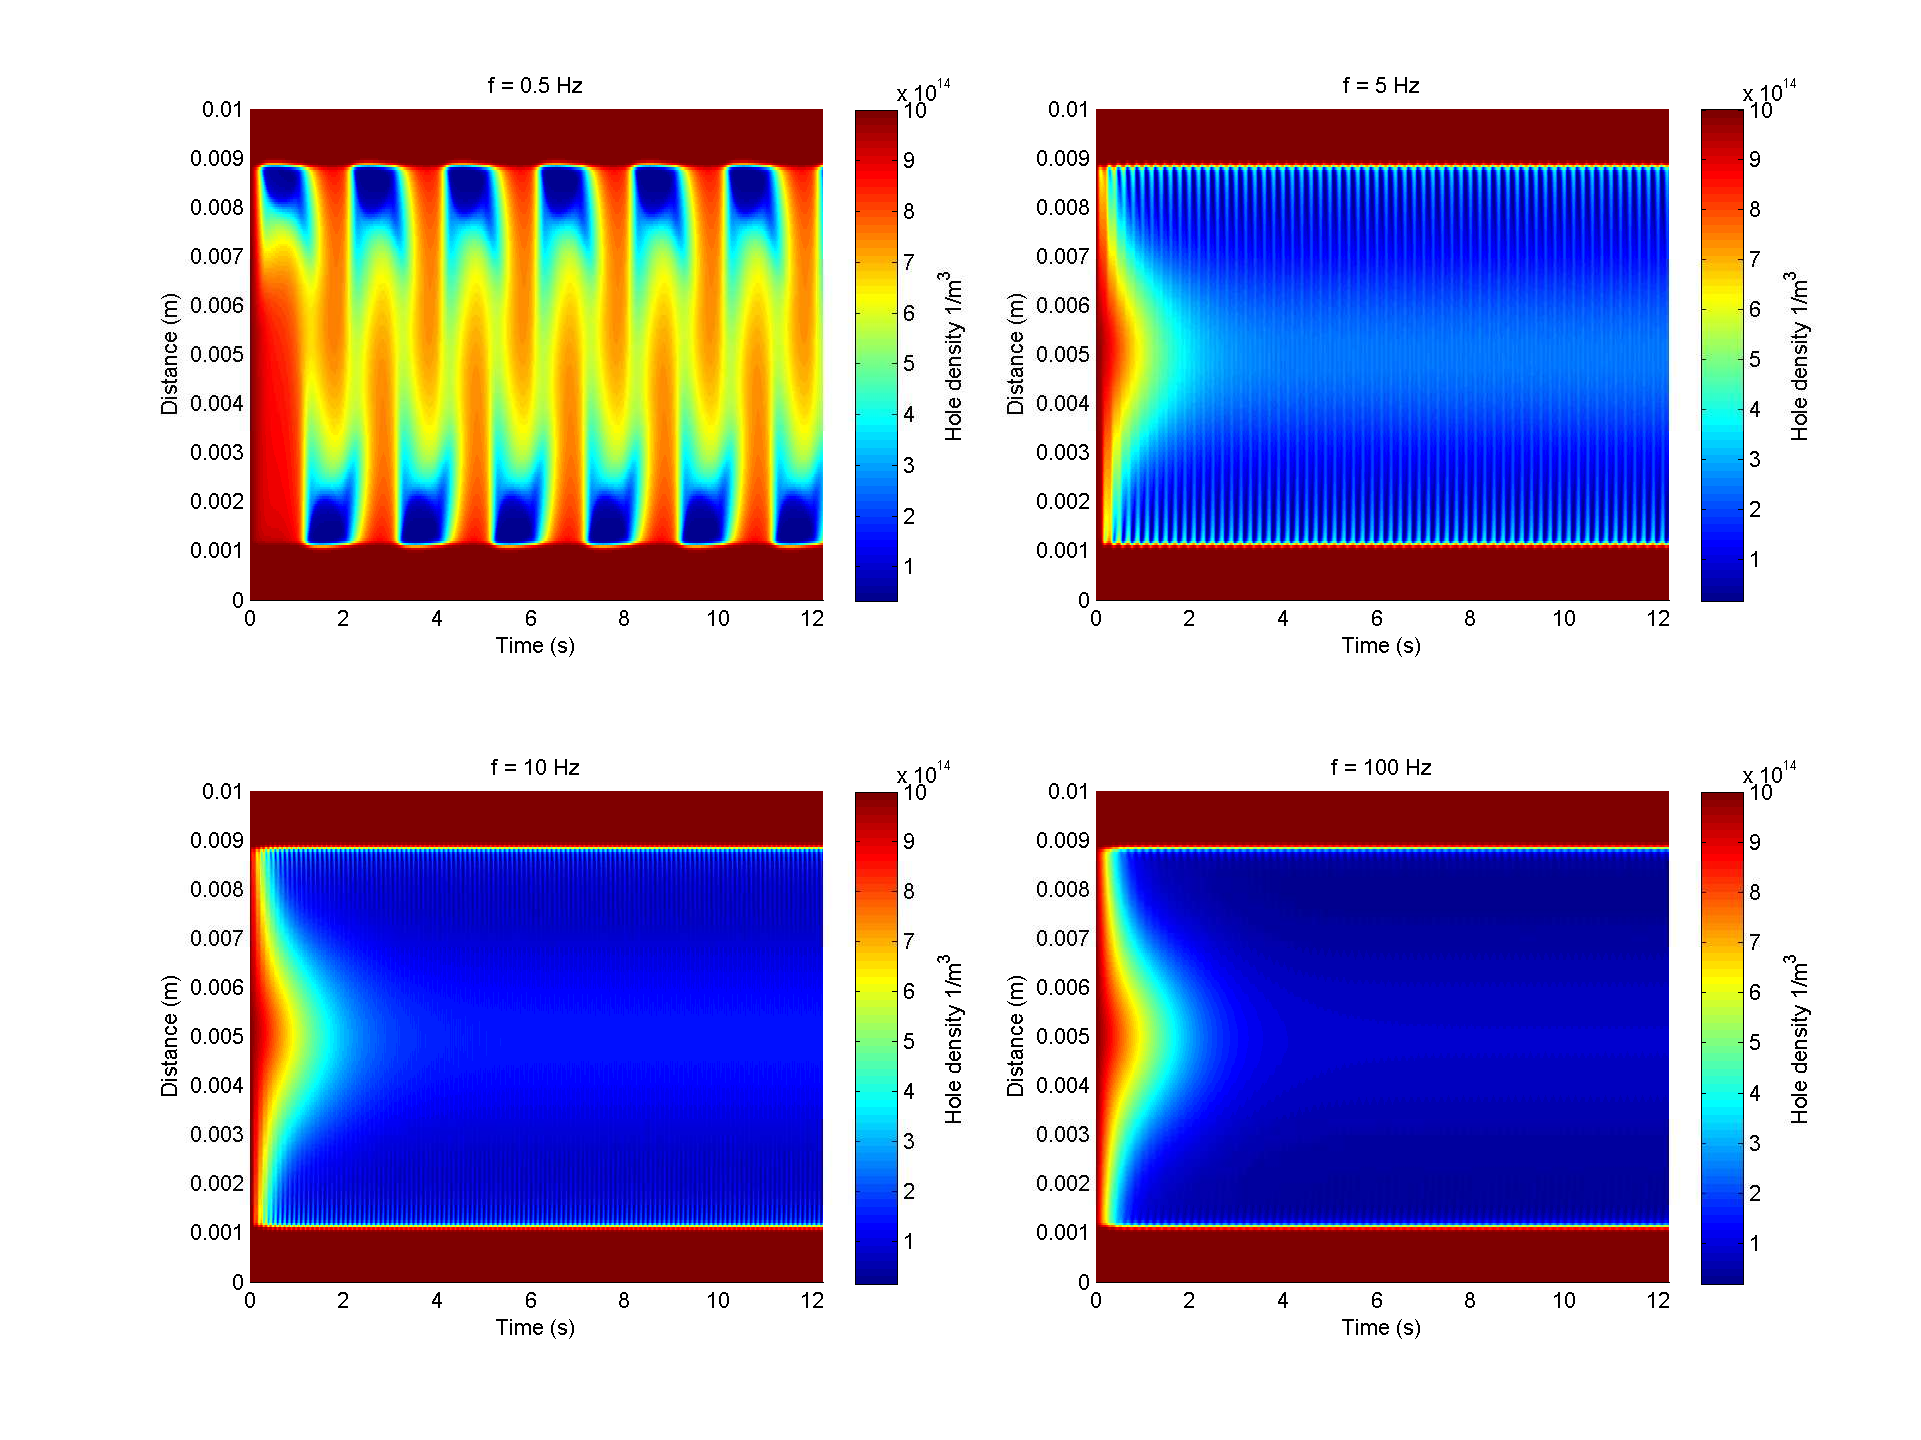
\includegraphics[scale=0.43]{1D_Memristor_Hole}
\caption{Hole density over time at different frequencies} 
\label{Bowhole}
\end{figure}

\begin{figure}[!htp]
\centering
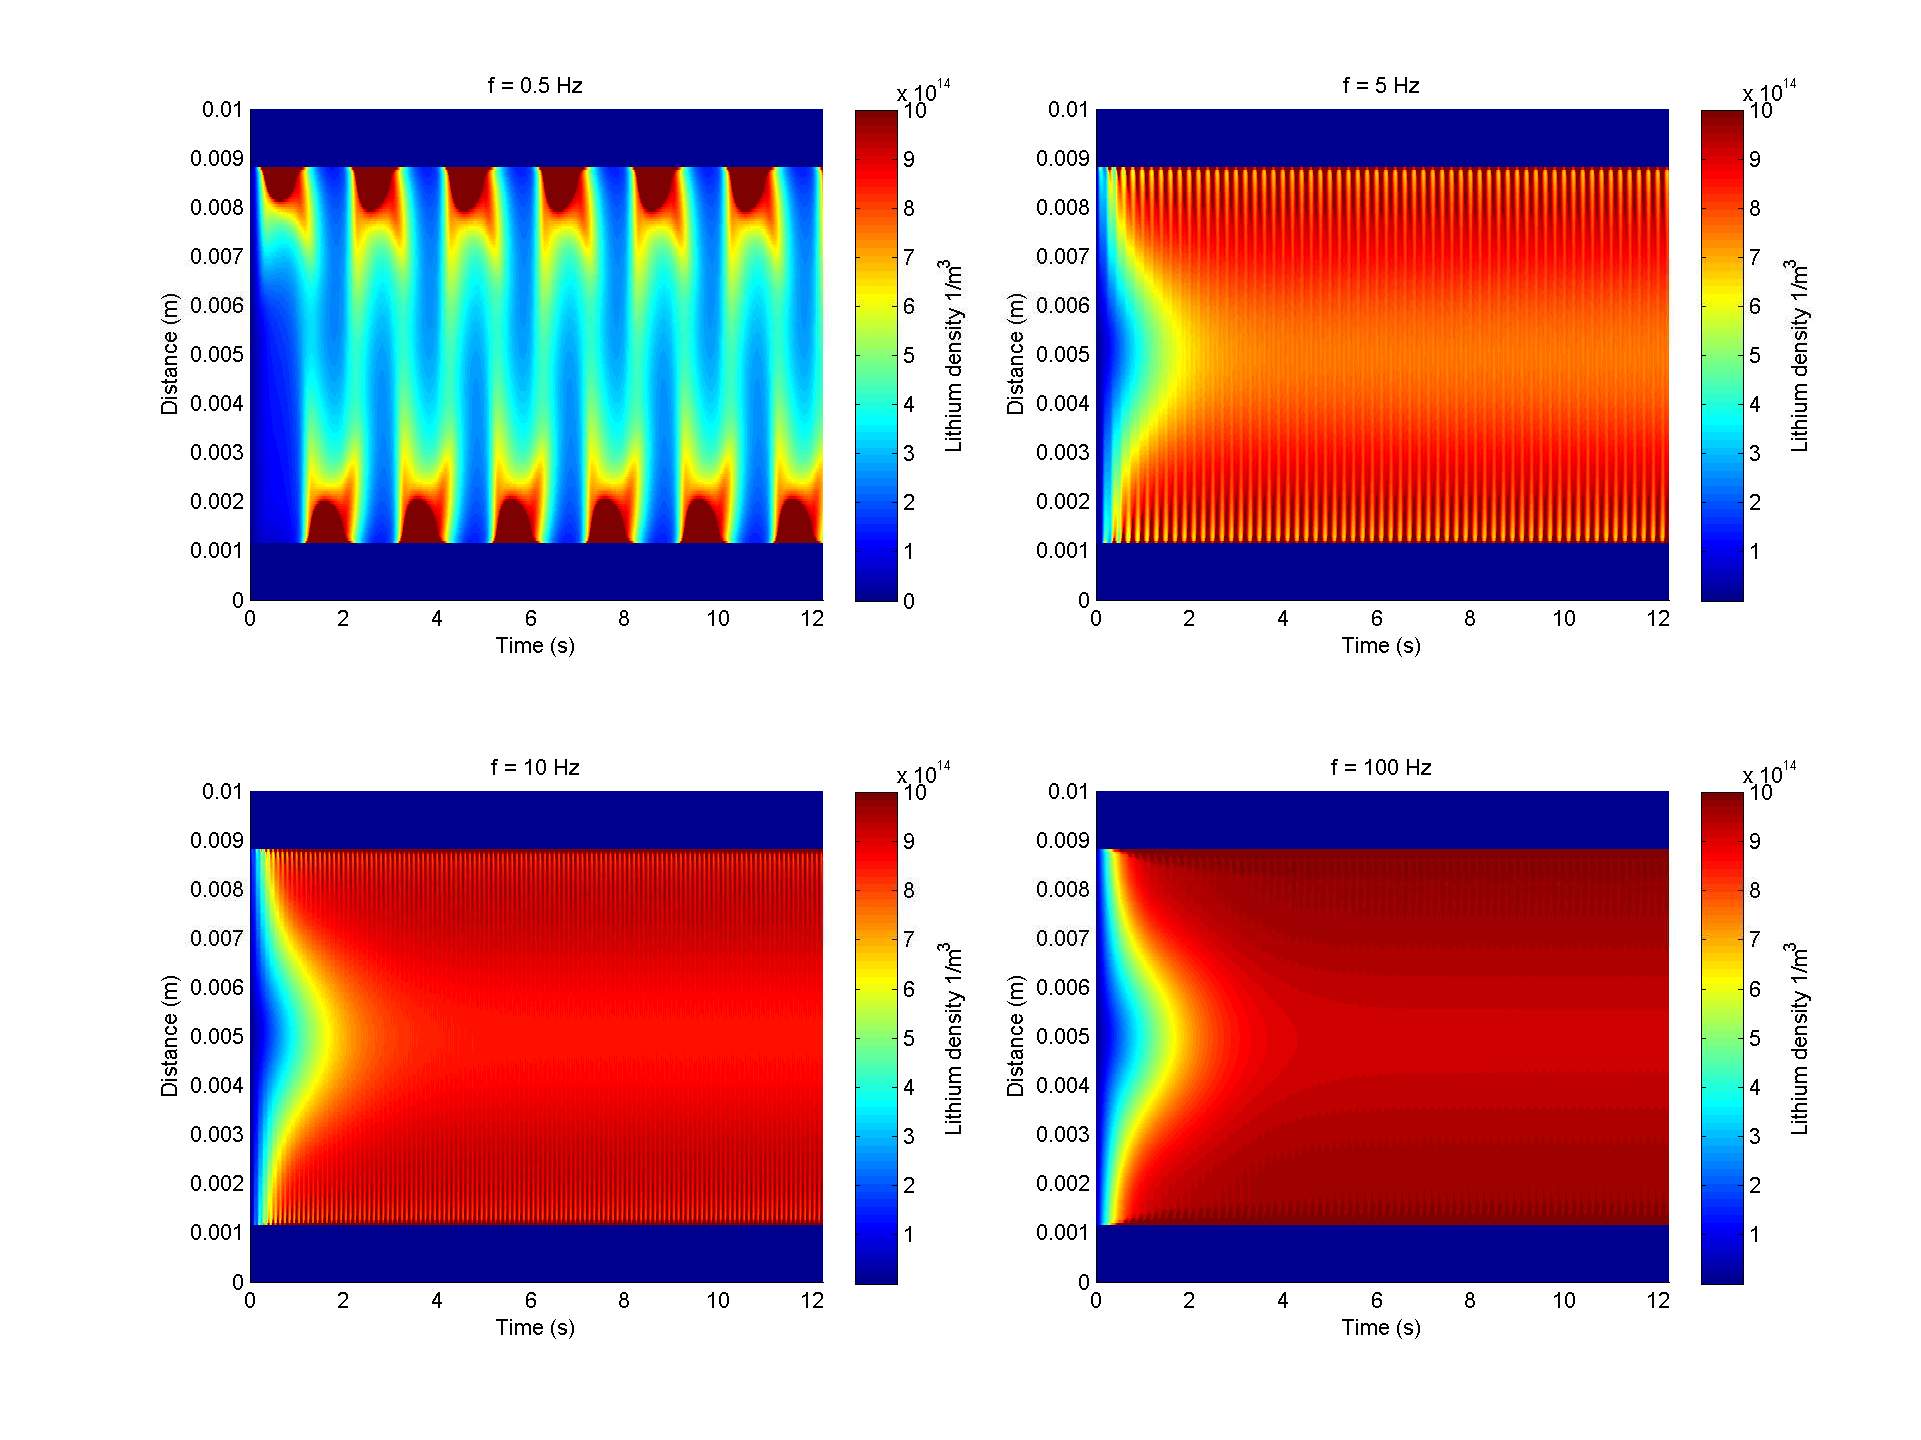
\includegraphics[scale=0.43]{1D_Memristor_Lithium}
\caption{Lithium density over time at different frequencies} 
\label{Bowli}
\end{figure}


\clearpage
\subsection{1-D Memristor Simulation With Increasing Charge Density}

After establishing that the simulation behaves as expected it is important to investigate how charge density effects this model. The model does not limit the particle density that can be simulated as long as the mesh density supports it but for the memristor the mesh density and the number of time steps required for the simulation becomes so large that the transient simulation cannot be completed in a reasonable amount of time using a standard computer. The actual device has a hole density in the range of $ \approx 10^{26}$ $m^{-3}$ but the simulation is restricted to $\approx 10^{17}$ $m^{-3}$ in this chapter. In theory, if the densities used for the simulation \tjsr{does}{} have a limited affect on the behavior of the memristor then the simulations with low particle densities can be use as a proxy for the actual device which operates in much higher particle densities.

 The following 3 figures (\ref{HoleDiff}, \ref{LithiumDiff} and \ref{DensityDiff}) show the hole and the lithium densities at steady state as well as the current density over time at the right metal contact for various charge densities. The simulations are run using high mesh densities to allow stable simulation up to $10^{17}$ $m^{-3}$. 20 different simulations were made using densities ranging from $5$ x $10^{15}$  $m^{-3}$ to 1 x $10^{17}$  $m^{-3}$ but only 5 of them are plotted for illustration purposes. All the values are normalized using respective hole/lithium density ratios. The following equations ares used for the normalization procedure.
\begin{equation}
\centering
n_{i}(x,t)^{'}= \frac{n_{i}(x,t)}{r_i} 
\end{equation}
\begin{equation}
\centering
J_{i}(t)^{'}= \frac{J_i(t)}{r_i} 
\end{equation}
\begin{equation}
\centering
r_i = \frac{n_{i}(x,t=0)}{n_{1}(x,t=0)}
\label{NormConst}
\end{equation}
%\tjs{where} $n_{i}$ is the charge carrier density which could be either holes or lithium ions depending on the plot. \textit{$J_{norm}$} is the normalized current density calculated at the right metal contact, \textit{r} is the normalization constant which is calculated using initial carrier density of the first plot ($n_{initial}$) of a simulation to be normalized and $n_{0}$ which is the carrier density of the initial plot ($5 x 10^{15}$ $m^{-3}$). After the normalization of various variables, all the plots are placed in the same graph to visually illustrate how increasing charge density affects the simulation. 

Where $n_{i}(x,t)^{'}$ and $J_{i}(t)^{'}$ are the particle and the current densities normalized by the coefficient $r_{i}$. This normalization coefficient is calculated by using the particle densities at $t=0$. 

$n_{1}(x,t=0)$ is the particle density of the plot with lowest initial hole or lithium density which is $5\;10^{15}\;1/m^3$ in this set of simulations. For example for a hole distribution with initial hole density at $65\;10^{15}\;1/m^3$ the normalization constant is,

\begin{equation}
\centering
r_i = \frac{n_{i}(x,t=0)}{n_{1}(x,t=0)} = \frac{65\;10^{15} }{5\;10^{15}} = 13
\label{NormConstVal}
\end{equation}

Once a transient simulation is complete the hole distribution is normalized using the normalization constant. A different normalization constant is calculated for every hole and lithium density and used to normalize the particle and current density distributions. The results are shown in figures \ref{LithiumDiff}, \ref{HoleDiff} and \ref{DensityDiff}. 
 
Plots for lithium ions (figure \ref{LithiumDiff}) and holes (figure \ref{HoleDiff}) are nearly identical to each other in terms of the plot shapes. They both get sharper around the area where there is a substantial accumulation of lithium ions. The debye length gets smaller with increasing carrier density. So with increased density it is expected that the density accumulation at the wet/dry PEDOT interface will be more narrow. This affect is not as strong for lithium ions because of density saturation. Lithium and hole plots only show the difference carrier density makes at steady state. The effect of debye length on the device operation can be further explored by looking at the current density over time.   

\begin{figure}[!htp]
\centering
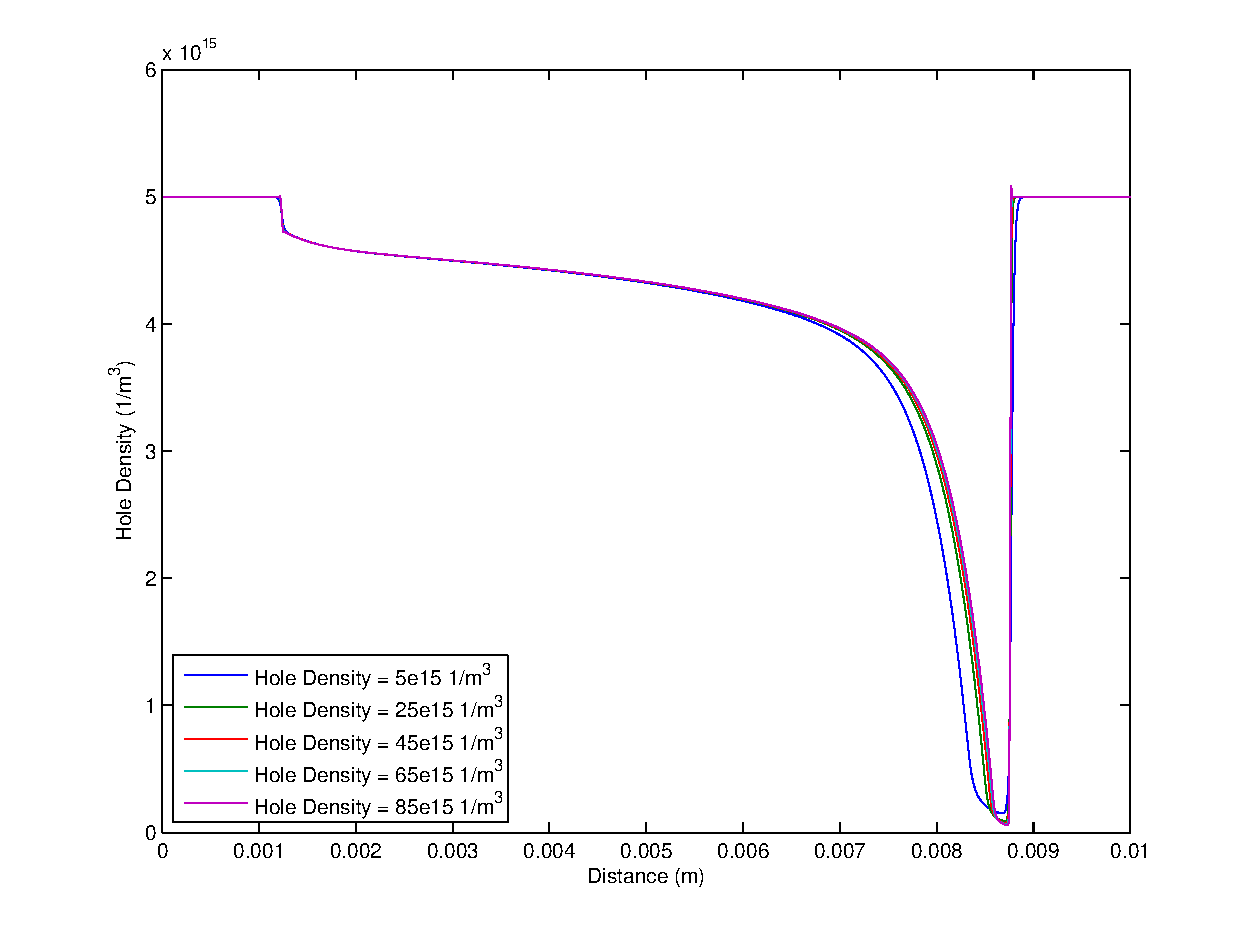
\includegraphics[scale=0.45]{HoleDiff}
\caption{Normalized hole densities at steady state} 
\label{HoleDiff}
\end{figure}

\begin{figure}[!htp]
\centering
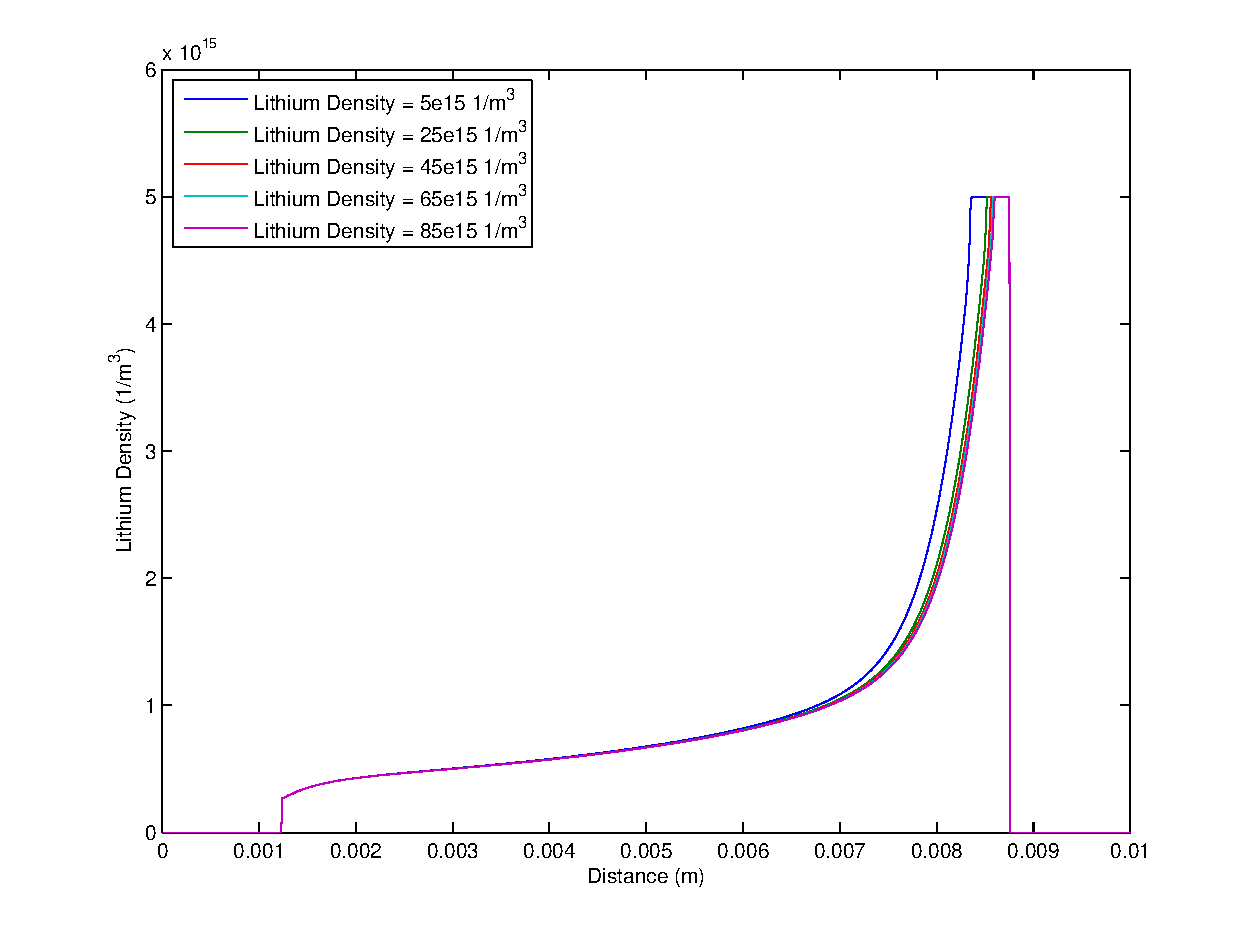
\includegraphics[scale=0.45]{LithiumDiff}
\caption{Normalized lithium densities at steady state} 
\label{LithiumDiff}
\end{figure}

\tjsr{F}{To investigate this the f}irst few milliseconds of \tjsr{this}{a} simulation is run without \tjs{allowing} the movement of lithium ions. At this stage normalized currents are identical to each other which means that a simulation with low density can be scaled up without introducing any errors. The introduction of lithium ions slowly deviates the current plots from each other over time but the overall behavior of the memristor remains unchanged. The current density decreases over time and reaches a steady state value. After the first plot which has the lowest hole density, consecutive plots get closer and they are almost impossible to distinguish from each other at steady state.

\begin{figure}[!htp]
\centering
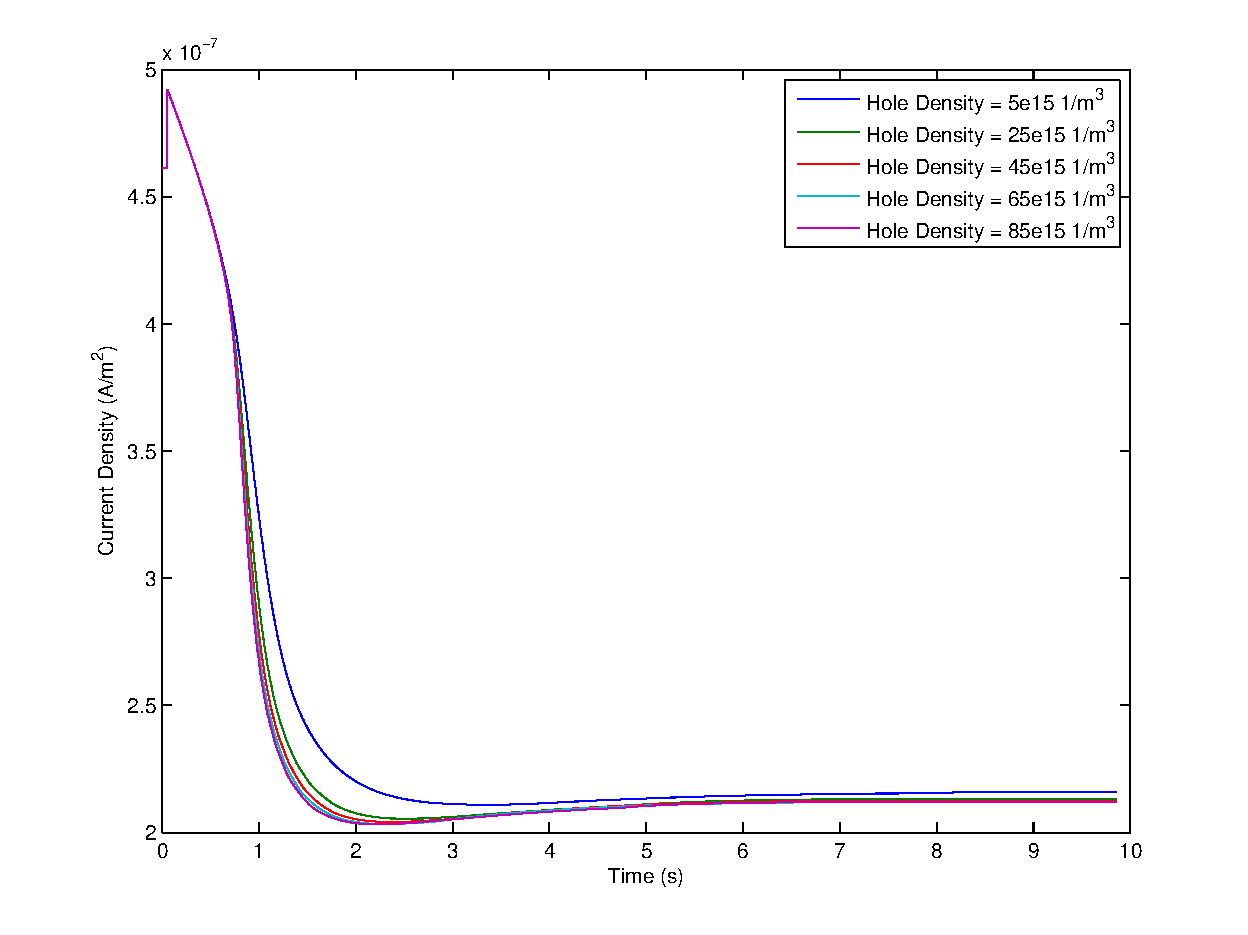
\includegraphics[scale=0.45]{DensityDiff}
\caption{Normalized hole current densities} 
\label{DensityDiff}
\end{figure}

 The normalized difference in the hole and lithium density distributions are not substantial and the overall shape of the plots are always preserved. The current density plots are also alike. Based on the plots above(\ref{HoleDiff},\ref{LithiumDiff} and \ref{DensityDiff}) it can be concluded that the behavior of the memristor simulated using a low charge density is very similar to the memristor simulation at a high charge density. This conclusion is also confirmed in section 7.4 where simulation results show comparable behavior to the experimental results.

\end{doublespace}


